\section{Configurazione dei connettori}
In questa sezione sono presenti delle schermate che illustrano la configurazione che è possibile fare per i singoli connettori aggiunti ad un workflow.
\label{sec:sec_conf_connettori_app}
\subsubsection{Configurazione connettore "Feed RSS"}
Il connettore "Feed RSS" permette di leggere delle news partendo dalla fonte specificata. Per aggiungere la fonte è presente un campo di testo come rappresentato nella seguente figura.
\begin{figure}[H]
	\centering
	%	\vspace*{-8cm}
	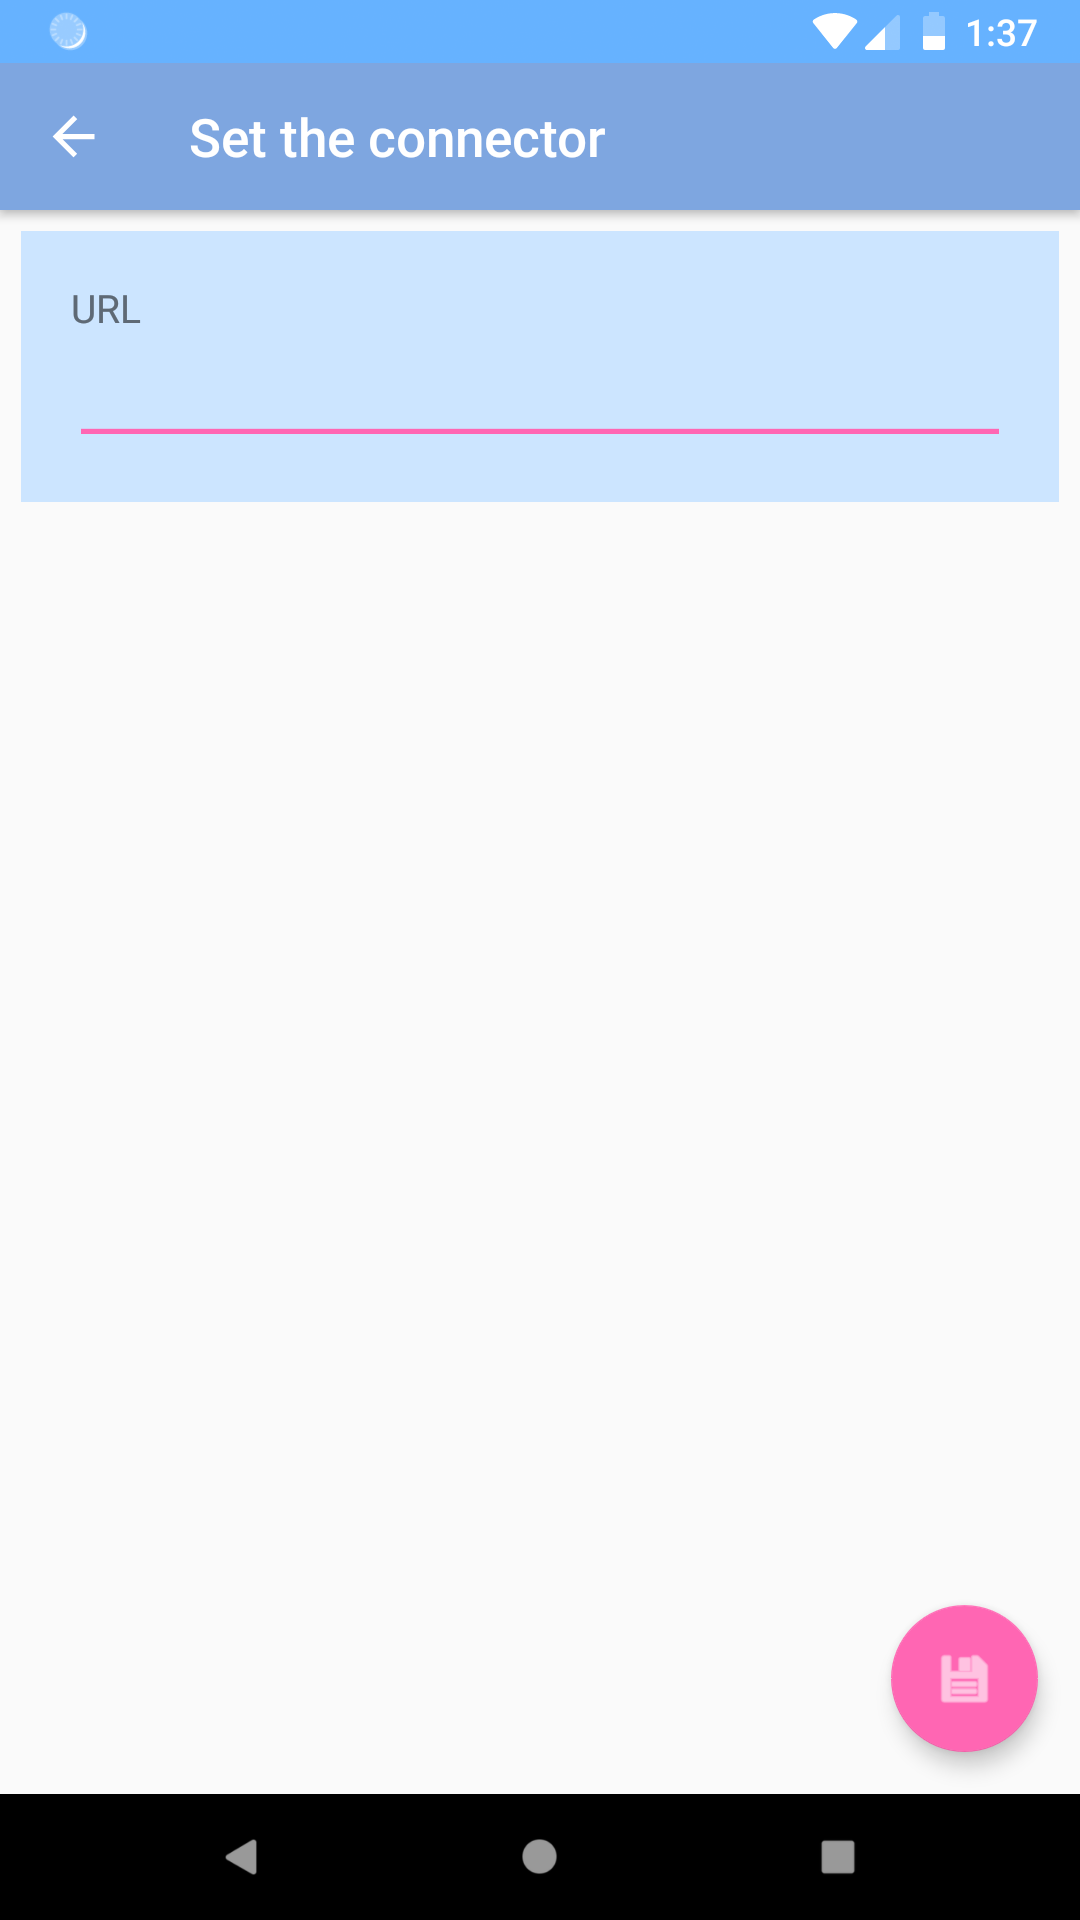
\includegraphics[width=5cm]{../includes/pics/configurazione_feed-rss.png}
	\caption{\label{fig:configurazione_feed-rss}Impostazione URL fonte Feed RSS}
\end{figure}
Per salvare le modifiche è sufficiente cliccare sul pulsante posto in fondo a destra della schermata.
\subsubsection{Configurazione connettore "Message"}
Il connettore "Message" permette di impostare un messaggio che l'assistente Alexa pronuncerà vocalmente. Per impostare il messaggio è presente un campo di testo come rappresentato nella seguente figura.
\begin{figure}[H]
	\centering
	%	\vspace*{-8cm}
	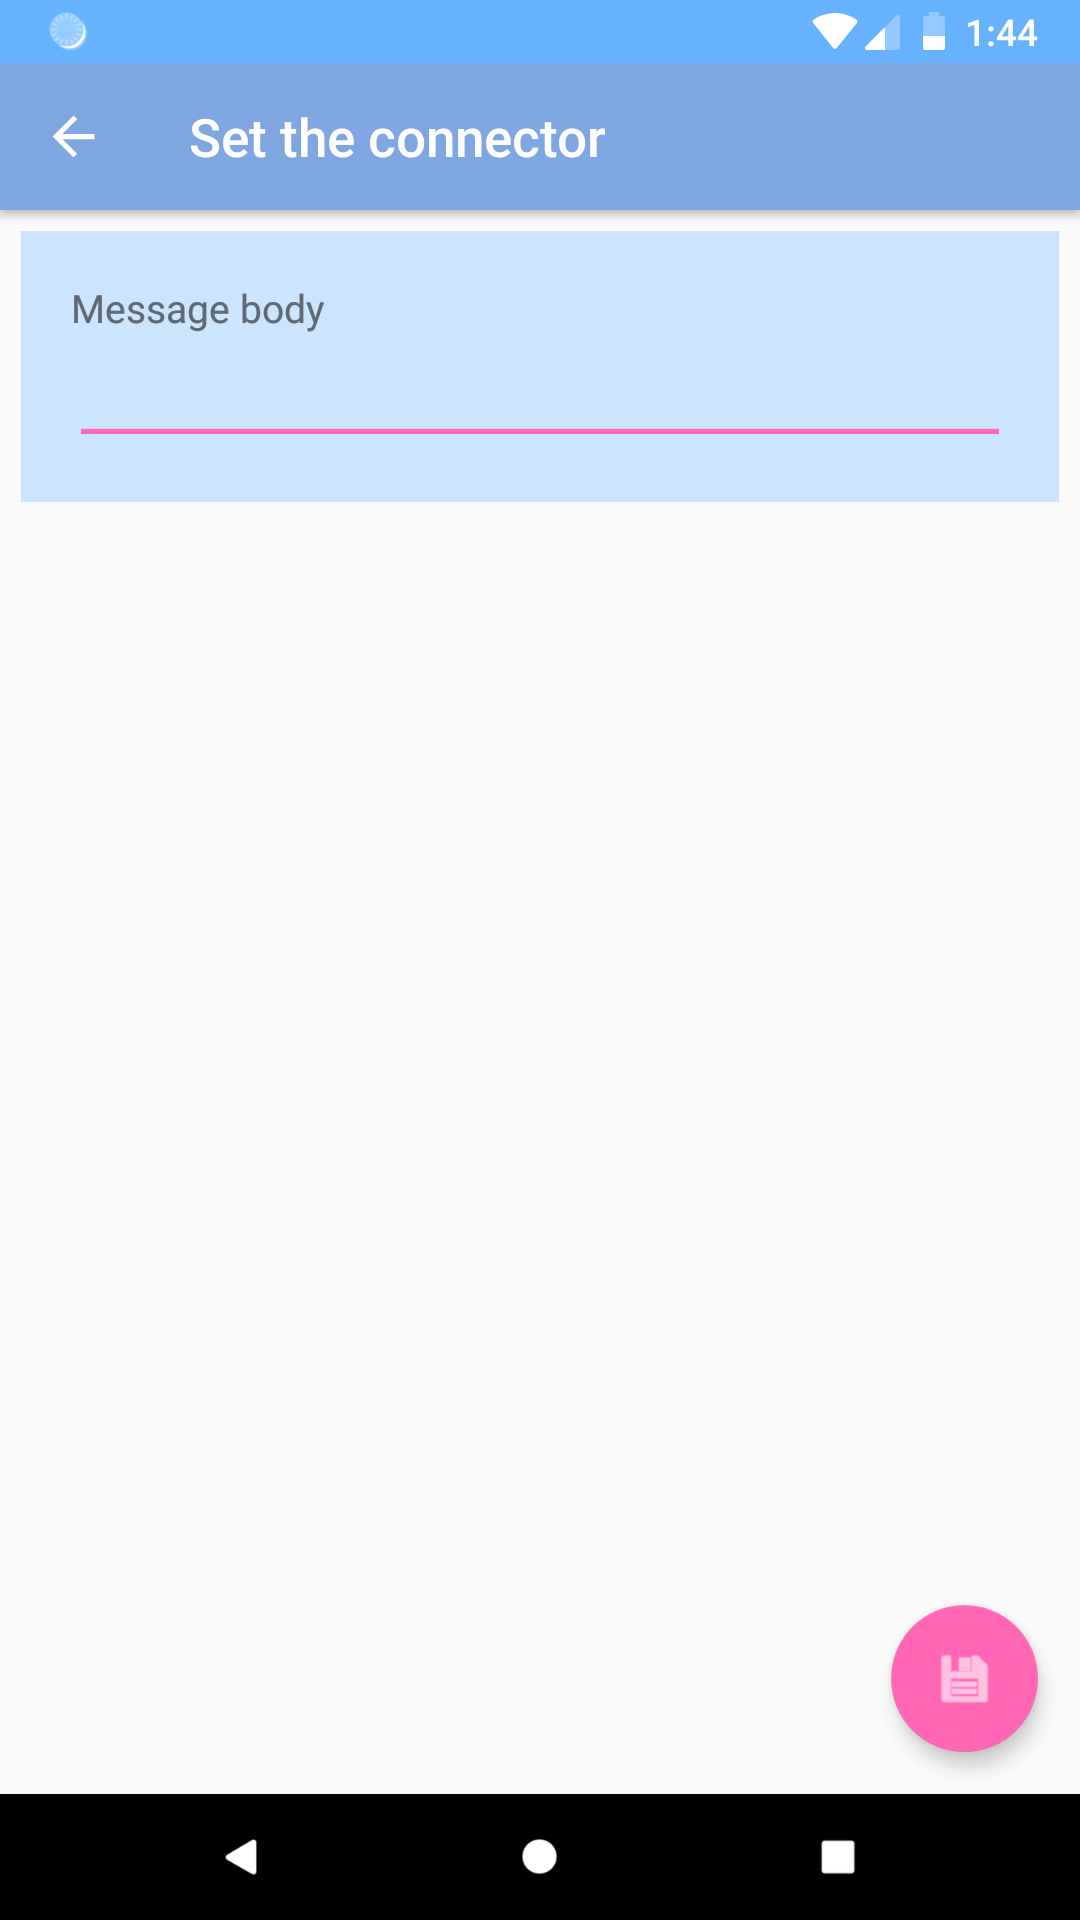
\includegraphics[width=5cm]{../includes/pics/configurazione_message-body.png}
	\caption{\label{fig:configurazione_message}Impostazione messaggio}
\end{figure}
Per salvare le modifiche è sufficiente cliccare sul pulsante posto in fondo a destra della schermata.

\subsection{Configurazione connettore "Weather"}
Il connettore "Weather" permette di ottenere informazioni sulle condizioni meteo di una località. Verrà chiesto di abilitare il GPS del telefono Android, in quanto in questo modo si riusciranno ad avere automaticamente le coordinate dell'utente.
Come si nota dalla figura sottostante, è anche possibile modificare a mano i due campi di testo "longitude" (longitudine) e "latitude" (latitudine).
\begin{figure}[H]
	\centering
	%	\vspace*{-8cm}
	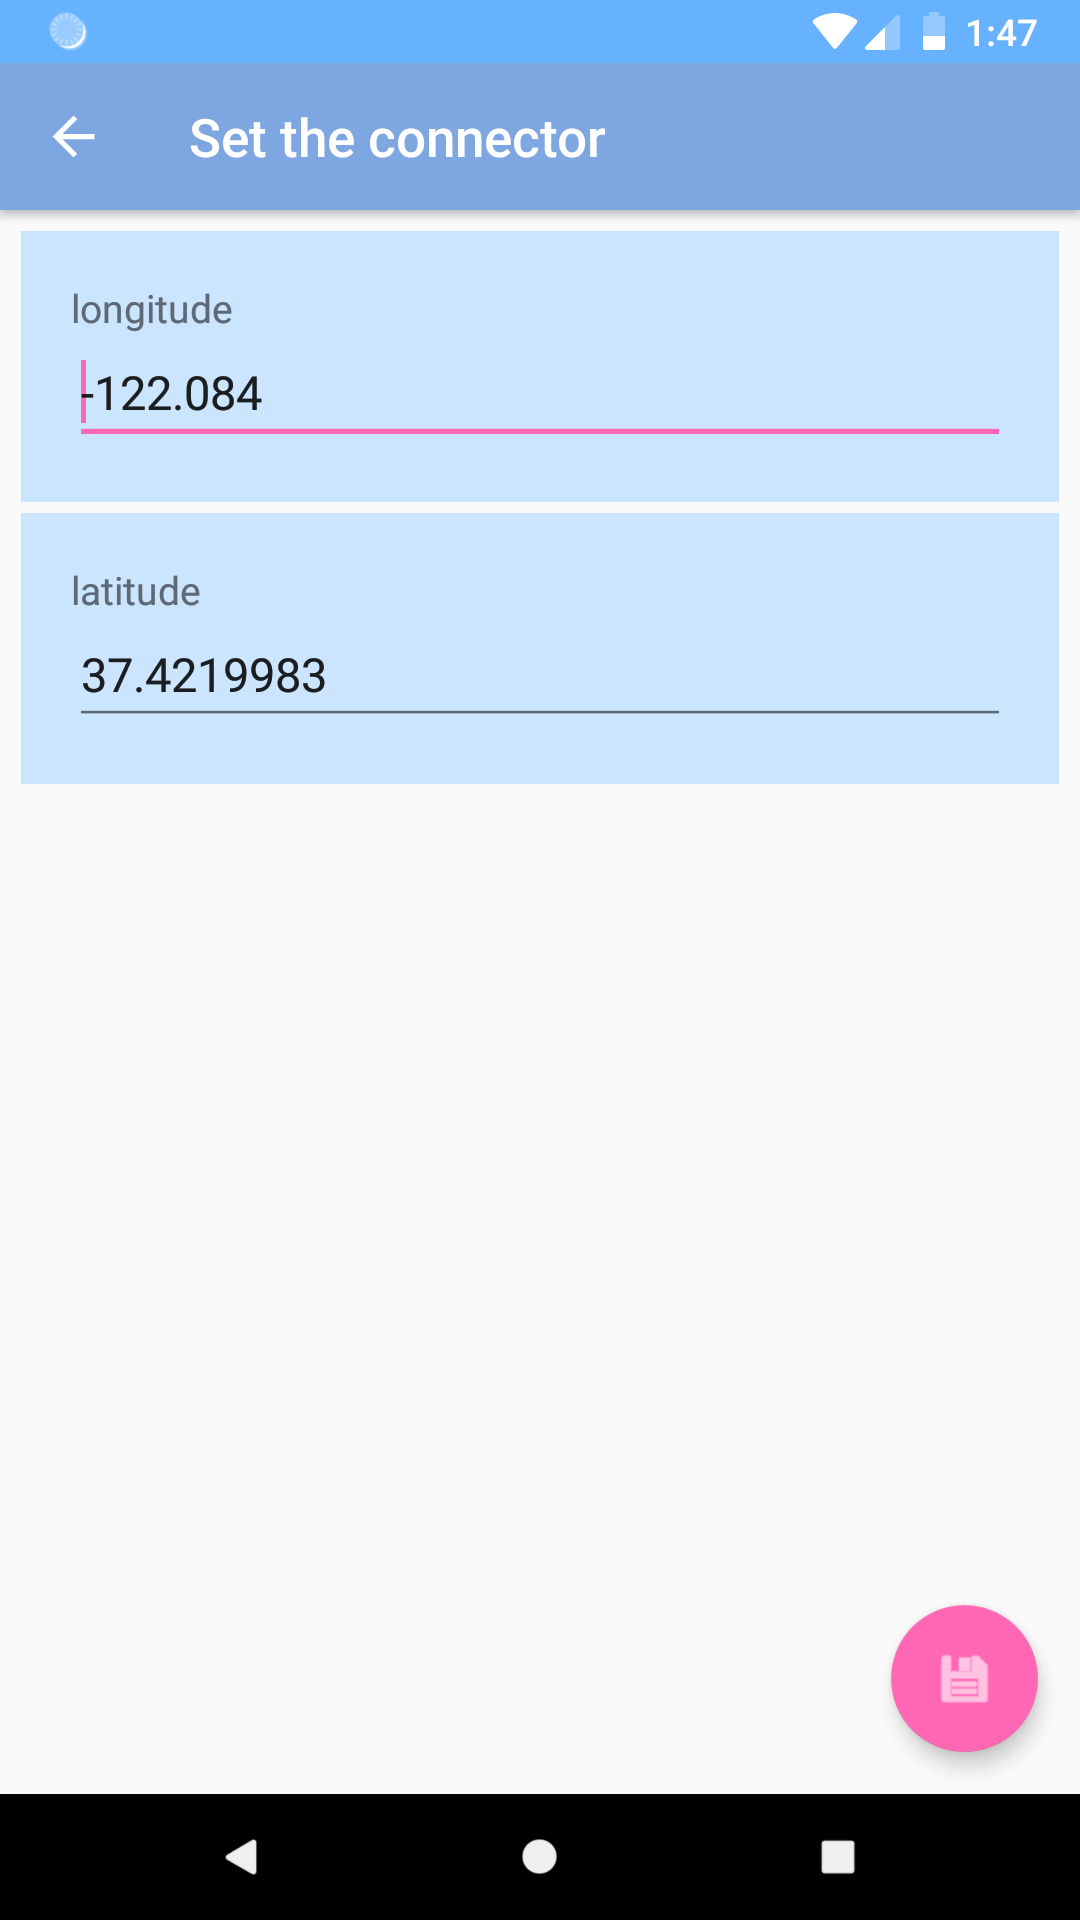
\includegraphics[width=5cm]{../includes/pics/configurazione_connettore_weather.png}
	\caption{\label{fig:configurazione_connettore_weather}Impostazione connettore "Weather"}
\end{figure}
Per salvare le modifiche è sufficiente cliccare sul pulsante posto in fondo a destra della schermata.

\subsubsection{Configurazione connettore "Read Tweets"}
Questo connettore permette di leggere gli ultimi 3 tweet pubblicati da un certo account di Twitter. A tal proposito è presente una casella di testo dove è possibile inserire lo username (es. "@unipd") relativo all'account desiderato.
\begin{figure}[H]
	\centering
	%	\vspace*{-8cm}
	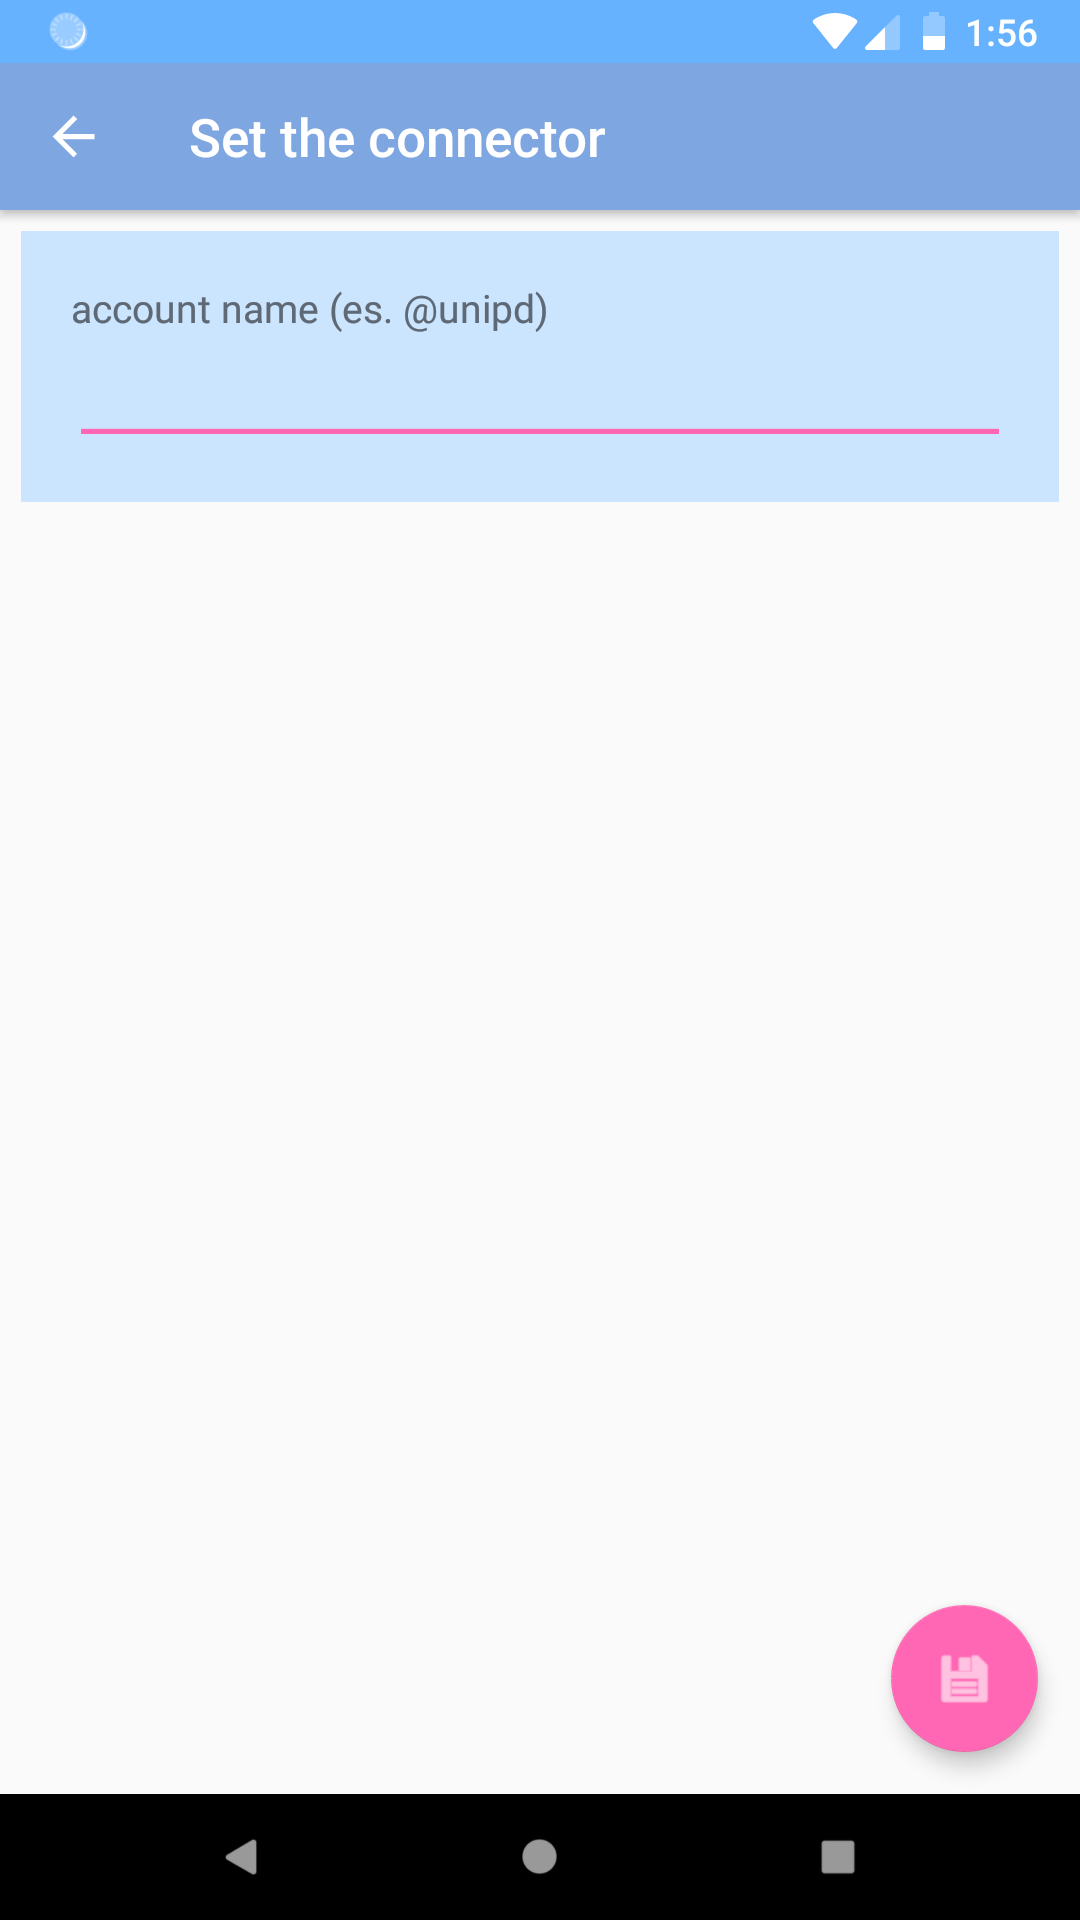
\includegraphics[width=5cm]{../includes/pics/conf_read_tweet.png}
	\caption{\label{fig:conf_read_tweet}Impostazione connettore "Read Tweets"}
\end{figure}
Per salvare le modifiche è sufficiente cliccare sul pulsante posto in fondo a destra della schermata.

\subsubsection{Configurazione connettore "Write Tweets"}
Questo connettore permette di pubblicare un tweet. Per poter usare questo connettore è necessario che l'utente faccia login al suo account di Twitter tramite il pulsante che compare.
E' necessario quindi seguire tutte le istruzioni che compaiono a schermo.
\begin{figure}[H]
	\centering
	%	\vspace*{-8cm}
	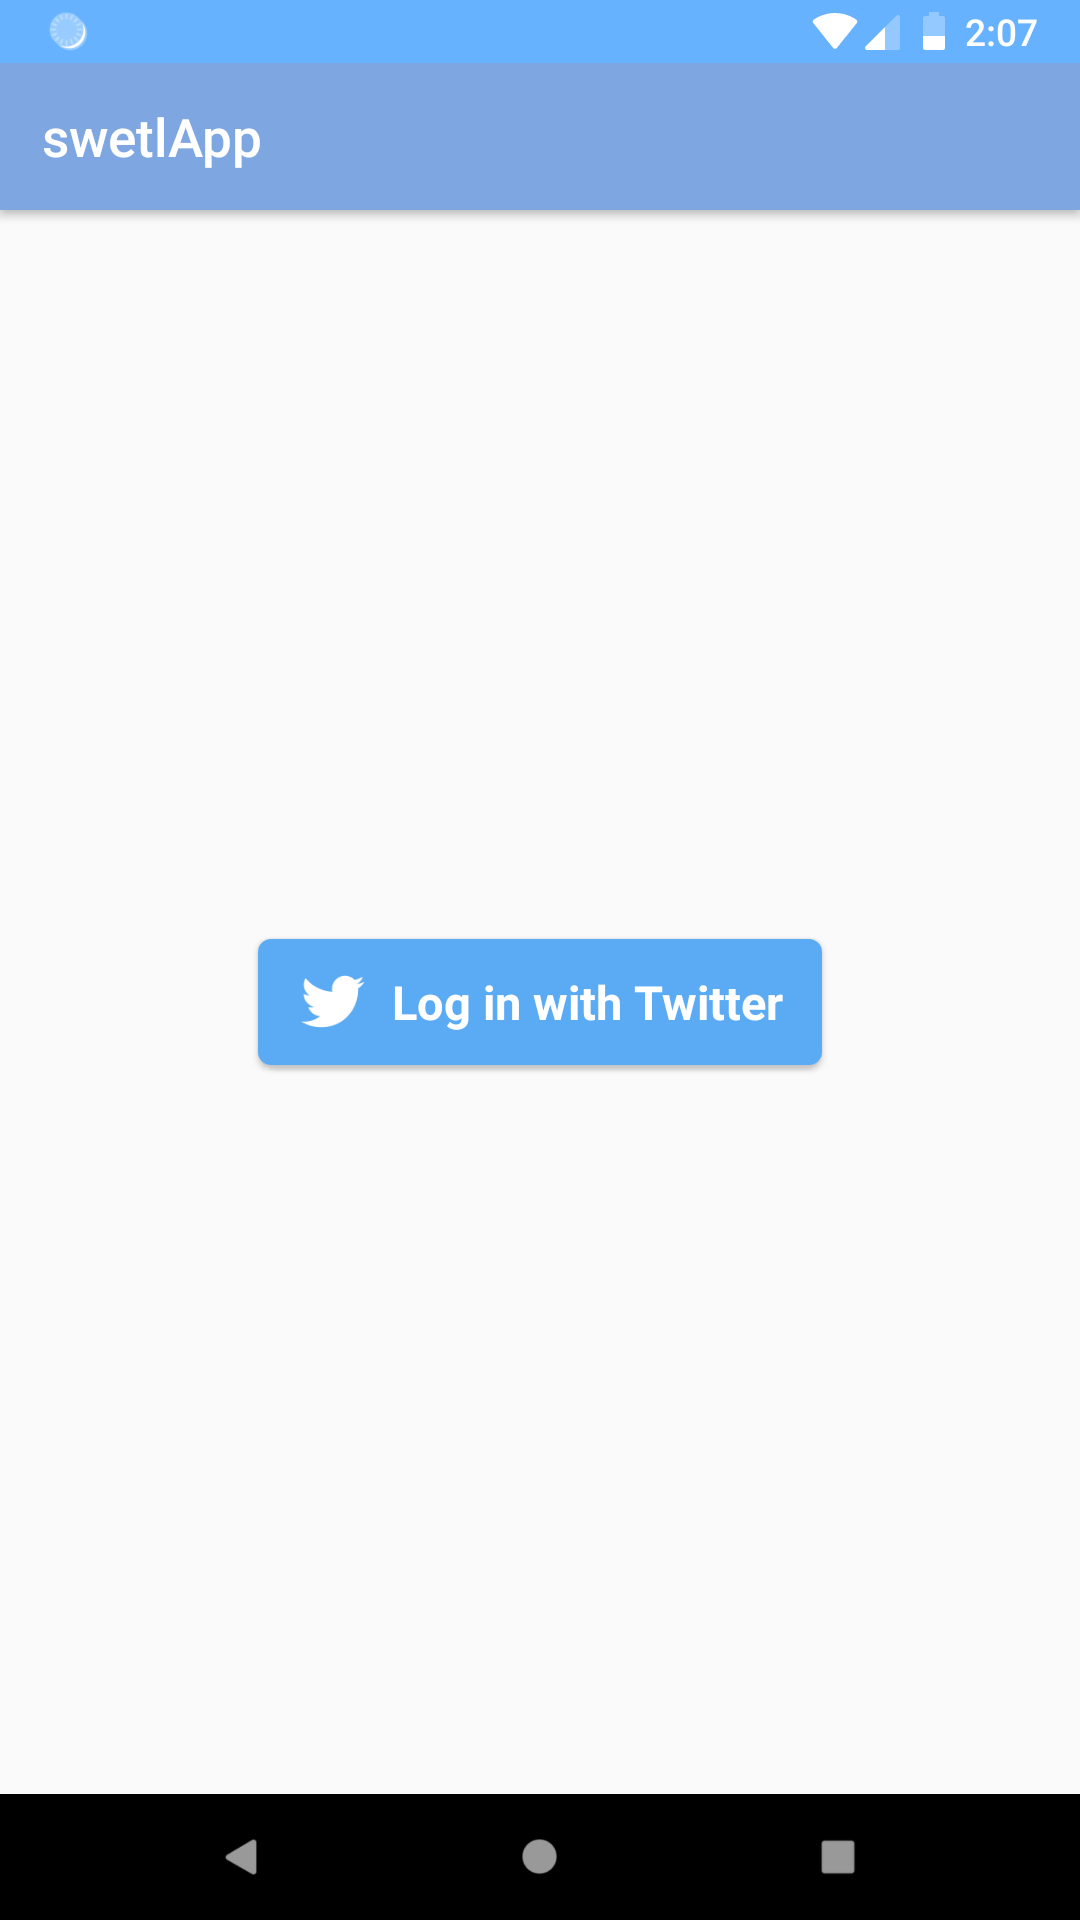
\includegraphics[width=5cm]{../includes/pics/conf_twitter_write.png}
	\caption{\label{fig:conf_twitter_write}Impostazione connettore "Write Tweets"}
\end{figure}


